\section{Optimizations}
Exploiting nested parallelism, is difficult on GPU hardware since the hardware is organized on one, or maybe two, levels that allow threads to comminucate via shared scratchpad memory. Hence mapping the application level parallelism to the GPU requires a choice of which level to paralellize, since both level cannot be directly mapped.\\
One way to get around this problem is to use a flattening transformation. The problem with this is that it will require even more memory usage, and may prevent opportunities for locality optimizations. We tried to do a flattening of our forawrd and backward rpoejctions, since we have multiple levels of paralellism. The idea was to compute the matrix, the transform it to a sparse and flat version and use our sparse matrix vector multiplication from a previous assignment. However, it turned out to be quite complex, and a lot of code was required to transform the matrix to the correct sparse format. Since it later turned out that most of the time spend during the computations was during the matrix computation and we had many issues with running out of memory, this probably wasn't the best approach and we did not pursue it to the end. We report result of semiflat versions.\\
A much more promising approach seems to be feeding the data directly to the matrix computations, and not have to save the matrix data at all but only the end result. We managed to finish an implementation of this approach for forward projection by feeding the data directly to the projectiomatrix\_doubleparallel version. Unfortunately, it ran out of resources so we need to investigate this further.\\
\begin{figure}[h]
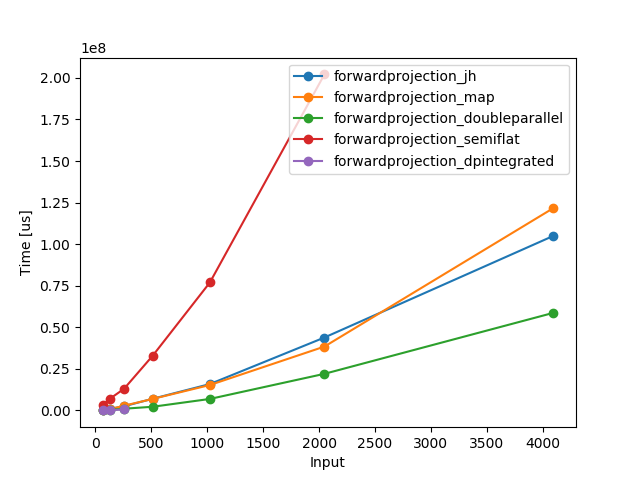
\includegraphics{images/forwardprojection_32.png}
\label{fpcompare}
  \caption{A comparison of the forward projections run with different matrix implementations and the version where the forward projection is integrated in projectiomatrix\_doubleparallel. The chunk size was 32. We chose this number to fit a CUDA warp. As expected the semiflat version performed rather badly. The implementation using the double parallel version performed best. The rest of the algorithms are nested, using different projection matrix algorithms inside. We had to run our algorithms for only 30 angles as we got memory errors otherwise. This requires further investigation. In our initial tests our stripmined algorithms ran for all sizes, but perhaps we were competing for space with other groups. }
\end{figure}
\begin{figure}[h]
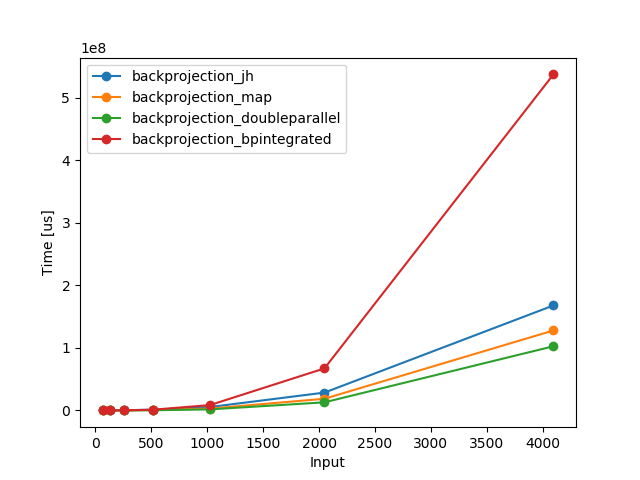
\includegraphics{images/backprojection_32.png}
\label{fpcompare}
  \caption{A comparison of the backprojections projections run with different matrix implementations and the version where the forward projection is integrated in projectiomatrix\_doubleparallel. The chunk size was 32. The implementation using the double parallel version of the matrix performed best again as expected. The integrated version performed very badly, and it would be interesting to investigate why. We had to run our algorithms for only 30 angles as we got memory errors otherwise.}
\end{figure}
\begin{figure}[h]
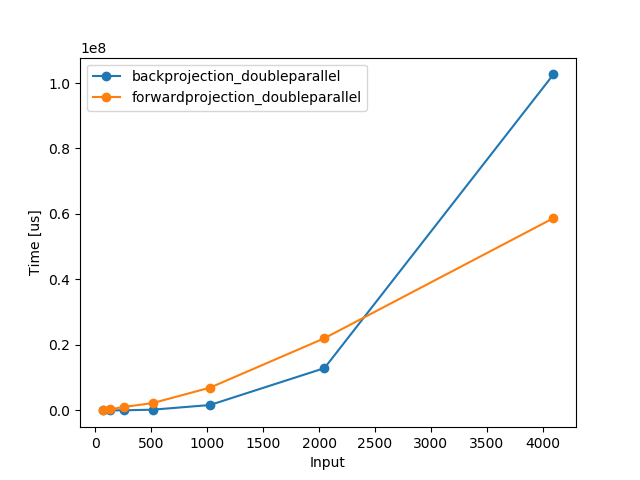
\includegraphics{images/backvsforwardprojection_32.png}
\label{fpcompare}
  \caption{A comparison of backprojection and forward projection. Backprojection seems to be faster for small problem sizes, but scale worse.}
\end{figure}
